\documentclass[norsk,a4paper,12pt]{article}
\usepackage[utf8]{inputenc}
\usepackage{graphicx} %for å inkludere grafikk
\usepackage{verbatim} %for å inkludere filer med tegn LaTeX ikke liker
\usepackage{tabularx}
\usepackage{booktabs}
\usepackage{amsmath}
\usepackage{float}
\usepackage{listings}
\usepackage{hyperref}
%\usepackage{subfigure}
\usepackage{subcaption}
\usepackage{caption}
\usepackage{color}
\usepackage[sep=3pt, offset=0.8em]{simpler-wick}
\usepackage{tikz}

\lstset{language=python}
\lstset{basicstyle=\small}
\lstset{backgroundcolor=\color{white}}
\lstset{frame=single}
\lstset{stringstyle=\ttfamily}
\lstset{keywordstyle=\color{red}\bfseries}
\lstset{commentstyle=\itshape\color{blue}}
\lstset{showspaces=false}
\lstset{showstringspaces=false}
\lstset{showtabs=false}
\lstset{breaklines}
\lstset{postbreak=\raisebox{0ex}[0ex][0ex]{\ensuremath{\color{red}\hookrightarrow\space}}}
%\usepackage{titlesec}

\setcounter{secnumdepth}{4}

%\titleformat{\paragraph}
%{\normalfont\normalsize\bfseries}{\theparagraph}{1em}{}
%\titlespacing*{\paragraph}
%{0pt}{3.25ex plus 1ex minus .2ex}{1.5ex plus .2ex}


\title{FYS-KJM4480 - Quantum mechanics for many-particle systems \\\vspace{2mm} \Large{Project 2}}
\author{\large Even Marius Nordhagen}
\date\today
\begin{document}

\maketitle

\begin{itemize}
\item For the Github repository containing programs and results, follow this link: 
\url{https://github.com/evenmn/master/tree/master/FYSKJM4480/Project2}
\end{itemize}

\section{Introduction}
Superconductivity might be one of 20th century's most exciting physical discoveries, and for a long time the theory behind was a mystery. In 1957, 46 years after the first observation by Kamerlingh Onnes [REFERENCE], John Bardeen, Leon Cooper and John Robert Schrieffer came up with a quantum theory describing superconductivity on microscopic level[REFERENCE]. This theory was built on Cooper pairs, which is a pair of electrons with lower energy than the Fermi energy, i.e. there is a bounding between them. We can treat the pairs as a particle, which is a boson due to the total spin 1, and this boson-like pair is the reason why the current can flow unhindered in a superconductor. 

Furthermore the theory is also used in nuclear physics to describe the paring interaction between nucleons in an atomic nucleus. 

This project aims to study such a pairing model, known as BCS-theory after its founders. In the first part we are working with this model independently. Then we will use Configuration-Interaction Doubled (CID) as an approximation to make the equations computer-friendly, and thereafter we repeat this using Coupled-Cluster Doubled (CCD). Finally the results are compared for both the methods, and we will discuss why one method is better than the other.
\newpage

\section{Pairing model}
In this project we use a slightly simplified pairing model, which we assume to be carrying a constant strength $g$. The Hamiltonian is therefore given by
\begin{equation}
\hat{H}=\hat{H}_0+\hat{V}
\end{equation}
with
\begin{equation}
\hat{H}_0=\sum_{p\sigma}\epsilon_pc_{p\sigma}^{\dagger}c_{p\sigma},\quad \epsilon_p=\xi\cdot(p-1)
\end{equation}
and
\begin{equation}
\hat{V}=-\frac{1}{2}g\sum_{pq}c_{p+}^{\dagger}c_{p-}^{\dagger}c_{q-}c_{q+}.
\end{equation}

We will only study systems of a even number of particles, $N$, and the ground-state wavefunction is then given by the Slater determinant
\begin{equation}
|\Phi\rangle=c_{1+}^{\dagger}c_{1-}^{\dagger}\hdots c_{N/2 +}^{\dagger}c_{N/2 -}^{\dagger}|\Phi\rangle.
\end{equation}
Further I will define some operators that will be useful when doing the calculations. 
\begin{equation}
\hat{P}_p^{\dagger}\equiv c_{p+}^{\dagger}c_{p-}^{\dagger},\quad \hat{P}_p\equiv c_{p-}c_{p+}
\end{equation}
\begin{equation}
\hat{n}_p\equiv\sum_{\sigma}c_{p\sigma}^{\dagger}c_{p\sigma}
\end{equation}
\begin{equation}
\hat{P}=\sum_p\hat{P}_p^{\dagger}\hat{P}_p
\end{equation}
and finally
\begin{equation}
\hat{S}_z=\frac{1}{2}\sum_{p\sigma}\sigma c_{p\sigma}^{\dagger}c_{p\sigma}.
\end{equation}

\subsection{Exercise 1A}
\subsection{Exercise 1B}
\subsection{Exercise 1C}
\subsection{Exercise 1D}
\begin{equation}
[\hat{P}_p,\hat{P}_q^{\dagger}]=\hat{P}_p\hat{P}_q^{\dagger}-\hat{P}_q^{\dagger}\hat{P}_p
\end{equation}
Will only include terms which contribute, and we obtain
\begin{align}
\hat{P}_p\hat{P}_q^{\dagger}&=\sum_{pq}c_{p-}c_{p+}c_{q+}^{\dagger}c_{q-}^{\dagger}\notag\\
&=\{c_{q+}^{\dagger}c_{q-}^{\dagger}c_{p-}c_{p+}\}+\{\wick{\c c_{p-}c_{p+}c_{q+}^{\dagger}\c c_{q-}^{\dagger}}\}+\{\wick{c_{p-}\c c_{p+}\c c_{q+}^{\dagger}c_{q-}^{\dagger}}\}+\{\wick{\c2 c_{p-}\c1 c_{p+}\c1 c_{q+}^{\dagger}\c2 c_{q-}^{\dagger}}\}\notag\\
&=\{c_{q+}^{\dagger}c_{q-}^{\dagger}c_{p-}c_{p+}\}-\delta_{pq}c_{p+}c_{q+}^{\dagger}-\delta_{pq}c_{p-}c_{q-}^{\dagger}+\delta_{pq}\delta_{pq}
\end{align}
due to Wick's theorem. Several terms vanish since a delta function of operators of opposite spin does not contribute, i.e. $\delta_{p+q-}=0$. Calculating $\hat{P}_q^{\dagger}\hat{P}_p$ is a simple task:
\begin{equation}
\hat{P}_q^{\dagger}\hat{P}_p=\{c_{q+}^{\dagger}c_{q-}^{\dagger}c_{p-}c_{p+}\}.
\end{equation}
Furthermore we will omit the spin in delta functions, because it does not affect the delta function as long as the spin is equally directed. We set $p=q$, but not in the Dirac delta functions:
\begin{align}
\hat{P}_p\hat{P}_q^{\dagger}-\hat{P}_q^{\dagger}\hat{P}_p&=-\delta_{pq}c_{q+}^{\dagger}c_{q+}-\delta_{pq}c_{q-}^{\dagger}c_{q-}+\delta_{pq}\delta_{qq}\notag\\
&=\delta_{pq}(1-c_{q+}^{\dagger}c_{q+}-c_{q-}^{\dagger}c_{q-})\notag\\
&=\delta_{pq}(1-\hat{n}_q)\label{eq:ex1d}
\end{align}

\subsection{e}
A fundamental property of the annihilation operator states that a such operator acting on the vacuum state becomes zero. This property will be used multiple times henceforce to get rid of terms, and the approach will often be to move the annihilation operator(s) such that this happens. 
We have $N=4$, thus 
\begin{align}
|\Phi\rangle&=c_{1+}^{\dagger}c_{1-}^{\dagger}c_{2+}^{\dagger}c_{2-}^{\dagger}|-\rangle\\
&=\hat{P}_1^{\dagger}\hat{P}_2^{\dagger}|-\rangle.
\end{align}
$M$ is the number of states, with $p$ as an index
\begin{align}
\hat{P}&=\sum_{p=1}^M\hat{P}_p^{\dagger}\hat{P}_p\\
&=\hat{P}_1^{\dagger}\hat{P}_1+\hat{P}_2^{\dagger}\hat{P}_2+\hat{P}_3^{\dagger}\hat{P}_3+\hat{P}_4^{\dagger}\hat{P}_4
\end{align}
since $M=4$. 
\begin{align}
\hat{P}|\Phi\rangle&=\Big(\hat{P}_1^{\dagger}\hat{P}_1\hat{P}_1^{\dagger}\hat{P}_2^{\dagger}+\hat{P}_2^{\dagger}\hat{P}_2\hat{P}_1^{\dagger}\hat{P}_2^{\dagger}+...\Big)|-\rangle\\
&=\Big(\delta_{11}\hat{P}_1^{\dagger}\hat{P}_2^{\dagger}+\delta_{22}\hat{P}_1^{\dagger}\hat{P}_2^{\dagger}\Big)|-\rangle\\
&=2|\Phi\rangle
\end{align}
where the two last terms in $\hat{P}$ do not contribute since $|\Phi\rangle$ does not contain creation operators with index 3 or 4. This computation was quite short since we could replace all operators with $\hat{P}$ which is not always the case, something we will see when calculating $\hat{S}_z|\Phi\rangle$.
\begin{align}
\hat{S}_z=&\frac{1}{2}\sum_{p\sigma}\sigma c_{p\sigma}^{\dagger}c_{p\sigma}\\
=&\frac{1}{2}\Big(c_{1+}^{\dagger}c_{1+}-c_{1-}^{\dagger}c_{1-}+c_{2+}^{\dagger}c_{2+}-c_{2-}^{\dagger}c_{2-}+\notag\\
&c_{3+}^{\dagger}c_{3+}-c_{3-}^{\dagger}c_{3-}+c_{4+}^{\dagger}c_{4+}-c_{4-}^{\dagger}c_{4-}\Big)|-\rangle
\end{align}
\begin{align}
\hat{S}_z|\Phi\rangle=&\frac{1}{2}\Big(c_{1+}^{\dagger}c_{1+}c_{1+}^{\dagger}c_{1-}^{\dagger}c_{2+}^{\dagger}c_{2-}^{\dagger}-c_{1-}^{\dagger}c_{1-}c_{1+}^{\dagger}c_{1-}^{\dagger}c_{2+}^{\dagger}c_{2-}^{\dagger}\notag\\
&+c_{2+}^{\dagger}c_{2+}c_{1+}^{\dagger}c_{1-}^{\dagger}c_{2+}^{\dagger}c_{2-}^{\dagger}-c_{2-}^{\dagger}c_{2-}c_{1+}^{\dagger}c_{1-}^{\dagger}c_{2+}^{\dagger}c_{2-}^{\dagger}\Big)|-\rangle\\
=&\frac{1}{2}\Big(\wick{c_{1+}^{\dagger}\c1 c_{1+}\c1 c_{1+}^{\dagger}c_{1-}^{\dagger}c_{2+}^{\dagger}c_{2-}^{\dagger}-c_{1-}^{\dagger}\c2 c_{1-}c_{1+}^{\dagger}\c2 c_{1-}^{\dagger}c_{2+}^{\dagger}c_{2-}^{\dagger}}\notag\\
&\wick{+c_{2+}^{\dagger}\c3 c_{2+}c_{1+}^{\dagger}c_{1-}^{\dagger}\c3 c_{2+}^{\dagger}c_{2-}^{\dagger}-c_{2-}^{\dagger}\c4 c_{2-}c_{1+}^{\dagger}c_{1-}^{\dagger}c_{2+}^{\dagger}\c4 c_{2-}^{\dagger}}\Big)|-\rangle\\
=&\frac{1}{2}\Big(\delta_{1+1+}c_{1+}^{\dagger}c_{1-}^{\dagger}c_{2+}^{\dagger}c_{2-}^{\dagger}-\delta_{1-1-}c_{1+}^{\dagger}c_{1-}^{\dagger}c_{2+}^{\dagger}c_{2-}^{\dagger}\notag\\\
&+\delta_{2+2+}c_{1+}^{\dagger}c_{1-}^{\dagger}c_{2+}^{\dagger}c_{2-}^{\dagger}-\delta_{2-2-}c_{1+}^{\dagger}c_{1-}^{\dagger}c_{2+}^{\dagger}c_{2-}^{\dagger}\Big)|-\rangle\\
=&\frac{1}{2}(1-1+1-1)|\Phi\rangle\\
=&0|\Phi\rangle
\end{align}

\subsection{f}
Observe that $|1\bar{1}2\bar{2}\rangle=|\Phi\rangle$.

\begin{figure*}
\begin{center}
  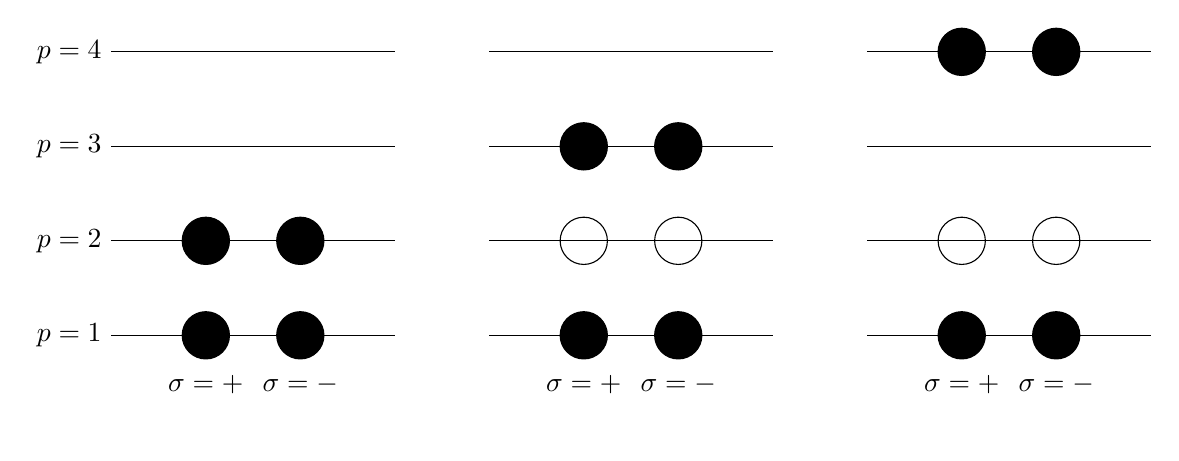
\begin{tikzpicture}[scale=1.2]
    \begin{scope}
      \foreach \i in {1,...,4}
      {
        \draw (-1,\i-1) node[anchor=east] {$p = \i$} --(2,\i-1);
      }
      \filldraw (0,0) node[anchor=north,inner sep=.5cm] {$\sigma=+$} circle (0.25cm); 
      \filldraw (1,0) node[anchor=north,inner sep=.5cm] {$\sigma=-$} circle (0.25cm);
      \filldraw (0,1) circle (0.25cm); 
      \filldraw (1,1) circle (0.25cm);
    \end{scope}
    \begin{scope}[xshift=4cm]
      \foreach \i in {1,...,4}
      {
        \draw (-1,\i-1) --(2,\i-1);
      }
      \filldraw (0,0) node[anchor=north,inner sep=.5cm] {$\sigma=+$} circle (0.25cm); 
      \filldraw (1,0) node[anchor=north,inner sep=.5cm] {$\sigma=-$} circle (0.25cm);
      \draw (0,1) circle (0.25cm); 
      \draw (1,1) circle (0.25cm);
      \filldraw (0,2) circle (0.25cm); 
      \filldraw (1,2) circle (0.25cm);
    \end{scope}
    \begin{scope}[xshift=8cm]
      \foreach \i in {1,...,4}
      {
        \draw (-1,\i-1) --(2,\i-1);
      }
      \filldraw (0,0) node[anchor=north,inner sep=.5cm] {$\sigma=+$} circle (0.25cm); 
      \filldraw (1,0) node[anchor=north,inner sep=.5cm] {$\sigma=-$} circle (0.25cm);
      \draw (0,1) circle (0.25cm); 
      \draw (1,1) circle (0.25cm);
      \filldraw (0,3) circle (0.25cm); 
      \filldraw (1,3) circle (0.25cm);
    \end{scope}
  \end{tikzpicture}
  \newline
  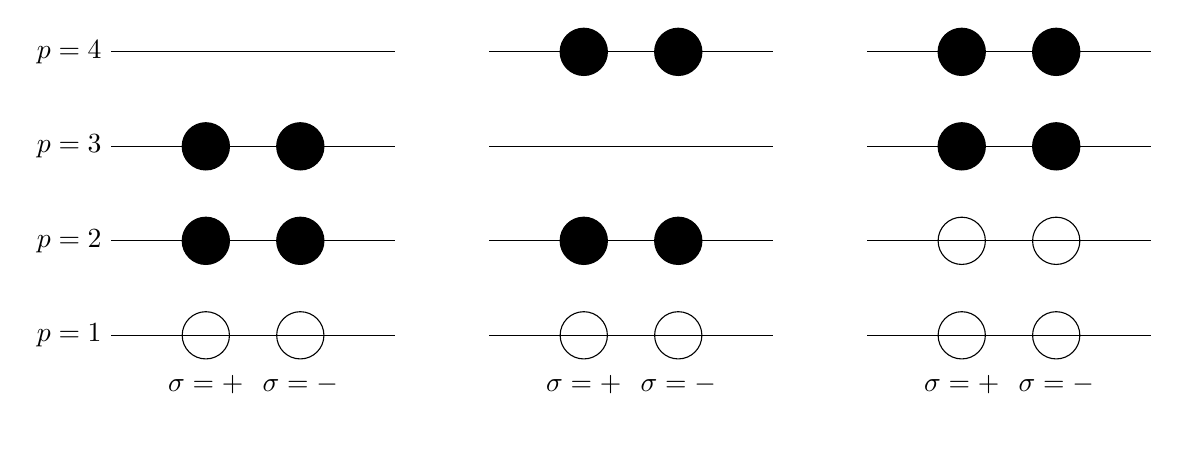
\begin{tikzpicture}[scale=1.2]
    \begin{scope}
      \foreach \i in {1,...,4}
      {
        \draw (-1,\i-1) node[anchor=east] {$p = \i$} --(2,\i-1);
      }
      \draw (0,0) node[anchor=north,inner sep=.5cm] {$\sigma=+$} circle (0.25cm); 
      \draw (1,0) node[anchor=north,inner sep=.5cm] {$\sigma=-$} circle (0.25cm);
      \filldraw (0,1) circle (0.25cm); 
      \filldraw (1,1) circle (0.25cm);
      \filldraw (0,2) circle (0.25cm); 
      \filldraw (1,2) circle (0.25cm);
    \end{scope}
    \begin{scope}[xshift=4cm]
      \foreach \i in {1,...,4}
      {
        \draw (-1,\i-1) --(2,\i-1);
      }
      \draw (0,0) node[anchor=north,inner sep=.5cm] {$\sigma=+$} circle (0.25cm); 
      \draw (1,0) node[anchor=north,inner sep=.5cm] {$\sigma=-$} circle (0.25cm);
      \filldraw (0,1) circle (0.25cm); 
      \filldraw (1,1) circle (0.25cm);
      \filldraw (0,3) circle (0.25cm); 
      \filldraw (1,3) circle (0.25cm);
    \end{scope}
    \begin{scope}[xshift=8cm]
      \foreach \i in {1,...,4}
      {
        \draw (-1,\i-1) --(2,\i-1);
      }
      \draw (0,0) node[anchor=north,inner sep=.5cm] {$\sigma=+$} circle (0.25cm); 
      \draw (1,0) node[anchor=north,inner sep=.5cm] {$\sigma=-$} circle (0.25cm);
      \draw (0,1) circle (0.25cm); 
      \draw (1,1) circle (0.25cm);
      \filldraw (0,2) circle (0.25cm); 
      \filldraw (1,2) circle (0.25cm);
      \filldraw (0,3) circle (0.25cm); 
      \filldraw (1,3) circle (0.25cm);
    \end{scope}
  \end{tikzpicture}
\end{center}
\caption{Need good caption here.\label{fig:schematic}}
\end{figure*}
From figure (\ref{fig:schematic}) one can observe that the dimension of the subspace for $M=4$ is $3+2+1=6$, which is the number of possible states. We can easily imagine that for $M=2$ we would get 1 state, with $M=5$ we would get $4+3+2+1=10$ states and so on. Thus the dimension of the subspace for an arbitrary $M$ is given by the arithmetic series
\begin{equation}
n_M=\sum_{m=1}^{M-1}(M-m).
\end{equation}

\subsection{1G}


\subsection{1H}
\begin{equation}
\hat{H}=\hat{H_0}+\hat{V}
\end{equation}
We use equation ... and ..., and get
\begin{align}
\hat{V}&=-\frac{1}{2}g\sum_{pq}c_{p+}^{\dagger}c_{p-}^{\dagger}c_{q-}c_{q+}\notag\\
&=-\frac{1}{2}g\sum_{p}^Mc_{p+}^{\dagger}c_{p-}^{\dagger}\sum_q^Mc_{q-}c_{q+}\notag\\
&=-\frac{1}{2}g\bigg(\sum_{p=1}^4\hat{P}_p^{\dagger}\bigg)\bigg(\sum_{q=1}^4\hat{P}_q\bigg)
\end{align}
Similarly we get
\begin{align}
\hat{H_0}&=\sum_{p\sigma}\varepsilon_pc_{p\sigma}^{\dagger}c_{p\sigma}\notag\\
&=\sum_p(p-1)\sum_{\sigma}c_{p\sigma}^{\dagger}c_{p\sigma}\notag\\
&=\sum_p(p-1)\hat{n}_p.
\end{align}
Thus we end up with
\begin{equation}
\hat{H}=\sum_p(p-1)\hat{n}_p-\frac{1}{2}g\bigg(\sum_{p=1}^4\hat{P}_p^{\dagger}\bigg)\bigg(\sum_{q=1}^4\hat{P}_q\bigg)
\end{equation}

\section{Configuration-Interaction (CI)}
\subsection{2A}
\begin{align}
\sum_s\hat{P}_s|p\bar{p}q\bar{q}\rangle=&\sum_s\hat{P}_s\hat{P}_p^{\dagger}\hat{P}_q^{\dagger}|-\rangle
\label{eq:2Aa}
\end{align}
We use the result from exercise 1D (equation(\ref{eq:ex1d})) twice, and get
\begin{align}
\hat{P}_s\hat{P}_p^{\dagger}\hat{P}_q^{\dagger}
=&\hat{P}_p^{\dagger}\hat{P}_s\hat{P}_q^{\dagger}+\delta_{sp}(1-\hat{n}_p)\hat{P}_q^{\dagger}\notag\\
=&\hat{P}_p^{\dagger}\hat{P}_q^{\dagger}\hat{P}_s+\hat{P}_p^{\dagger}\delta_{sq}(1-\hat{n}_q)+\delta_{sp}(1-\hat{n}_p)\hat{P}_q^{\dagger}
\end{align}
Then insert back into equation (\ref{eq:2Aa}):
\begin{align}
&\sum_s(\hat{P}_p^{\dagger}\hat{P}_q^{\dagger}\hat{P}_s+\hat{P}_p^{\dagger}\delta_{sq}(1-\hat{n}_q)+\delta_{sp}(1-\hat{n}_p)\hat{P}_q^{\dagger})|-\rangle\notag\\
&=\sum_s(\hat{P}_p^{\dagger}\delta_{sq}(1-\hat{n}_q)+\delta_{sp}(1-\hat{n}_p)\hat{P}_q^{\dagger})|-\rangle\notag\\
&=\sum_s(\delta_{sq}\hat{P}_p^{\dagger}-\delta_{sq}\hat{P}_p^{\dagger}\hat{n}_q+\delta_{sp}\hat{P}_q^{\dagger}-\delta_{sp}\hat{n}_p\hat{P}_q^{\dagger})|-\rangle\notag\\
&=\sum_s(\delta_{sp}\hat{P}_p^{\dagger}+\delta_{sq}\hat{P}_q^{\dagger})|-\rangle\notag\\
&=(\hat{P}_p^{\dagger}+\hat{P}_q^{\dagger})|-\rangle\notag\\
&=|p\bar{p}\rangle+|q\bar{q}\rangle
\end{align}
Firstly the first term vanishes, since an annihilation operator acts on the vacuum. Also when $\hat{n}_p$ acts on vacuum the term dies, and since this operator is hermitian, it can always be moved to the vacuum. Further we will find the Hamiltonian matrix
\begin{equation}
\langle p'\bar{p}'q'\bar{q}|\hat{H}|p\bar{p}q\bar{q}\rangle=\langle p'\bar{p}'q'\bar{q}|\hat{H}_0|p\bar{p}q\bar{q}\rangle+\langle p'\bar{p}'q'\bar{q}|\hat{V}|p\bar{p}q\bar{q}\rangle
\end{equation}
I will start with the first one:
\begin{equation}
\hat{H}_0|p\bar{p}q\bar{q}\rangle = \sum_{r\sigma}\epsilon_rc_{r\sigma}^{\dagger}c_{r\sigma}c_{p+}^{\dagger}c_{p-}^{\dagger}c_{q+}^{\dagger}c_{q-}^{\dagger}|-\rangle
\end{equation}
I will use Wick's theorem to calculate this, and since requires normal ordering, the vacuum state will kill all strings including an annihilation operator. In this case we therefore get four terms which come from single contraction. We will get delta functions, which only contribute when both indexes are equal, so for instance if we get $\delta_{rp}$ we need to set $r=p$ since $r$ runs over all possible states.
\begin{align}
\hat{H}_0|p\bar{p}q\bar{q}\rangle =& \sum_{r\sigma}\epsilon_r\{c_{r\sigma}^{\dagger}c_{p+}^{\dagger}c_{p-}^{\dagger}c_{q+}^{\dagger}c_{q-}^{\dagger}c_{r\sigma}\}|-\rangle\notag\\
&+\sum_{r\sigma}\epsilon_r\delta_{r\sigma p+}c_{r\sigma}^{\dagger}c_{p-}^{\dagger}c_{q+}^{\dagger}c_{q-}^{\dagger}|-\rangle\notag\\
&-\sum_{r\sigma}\epsilon_r\delta_{r\sigma p-}c_{r\sigma}^{\dagger}c_{p+}^{\dagger}c_{q+}^{\dagger}c_{q-}^{\dagger}|-\rangle\notag\\
&+\sum_{r\sigma}\epsilon_r\delta_{r\sigma q+}c_{r\sigma}^{\dagger}c_{p+}^{\dagger}c_{p-}^{\dagger}c_{q-}^{\dagger}|-\rangle\notag\\
&-\sum_{r\sigma}\epsilon_r\delta_{r\sigma q-}c_{r\sigma}^{\dagger}c_{p+}^{\dagger}c_{p-}^{\dagger}c_{q+}^{\dagger}|-\rangle\\
=&(\epsilon_pc_{p+}^{\dagger}c_{p-}^{\dagger}c_{q+}^{\dagger}c_{q-}^{\dagger}-\epsilon_pc_{p-}^{\dagger}c_{p+}^{\dagger}c_{q+}^{\dagger}c_{q-}^{\dagger}\notag\\
&+\epsilon_qc_{q+}^{\dagger}c_{p+}^{\dagger}c_{p-}^{\dagger}c_{q-}^{\dagger}-\epsilon_qc_{q-}^{\dagger}c_{p+}^{\dagger}c_{p-}^{\dagger}c_{q+}^{\dagger})|-\rangle\\
=&(\epsilon_pc_{p+}^{\dagger}c_{p-}^{\dagger}c_{q+}^{\dagger}c_{q-}^{\dagger}+\epsilon_pc_{p+}^{\dagger}c_{p-}^{\dagger}c_{q+}^{\dagger}c_{q-}^{\dagger}\notag\\
&+\epsilon_qc_{p+}^{\dagger}c_{p-}^{\dagger}c_{q+}^{\dagger}c_{q-}^{\dagger}+\epsilon_qc_{p+}^{\dagger}c_{p-}^{\dagger}c_{q+}^{\dagger}c_{q-}^{\dagger})|-\rangle\\
=&2(\epsilon_p+\epsilon_q)(\hat{P}_p^{\dagger}\hat{P}_p^{\dagger})|-\rangle\\
=&2(2-p-q)|p\bar{p}q\bar{q}\rangle
\end{align} 
where $\xi=1$ is assumed. We then get
\begin{equation}
\langle p'\bar{p}'q'\bar{q}'|\hat{H}_0|p\bar{p}q\bar{q}\rangle=2(2-p-q)\langle p'\bar{p}'q'\bar{q}'|p\bar{p}q\bar{q}\rangle
\end{equation}
So we still need to calculate the braket (Puh)
\begin{equation}
\langle p'\bar{p}'q'\bar{q}'|p\bar{p}q\bar{q}\rangle=\langle-|\hat{P}_{p'}\hat{P}_{q'}\hat{P}_p^{\dagger}\hat{P}_q^{\dagger}|-\rangle
\end{equation}
Again we will try to move the annihilation operator all the way to the right, such that it acts on the vacuum. The result from exercise 1D will be applied several times.
\begin{align}
\hat{P}_{p'}\hat{P}_{q'}\hat{P}_p^{\dagger}\hat{P}_q^{\dagger}&=\hat{P}_{p'}\hat{P}_p^{\dagger}\hat{P}_{q'}\hat{P}_q^{\dagger}+\delta_{q'p}\hat{P}_{p'}(1-\hat{n}_p)\hat{P}_q^{\dagger}\\
&=\hat{P}_{p'}\hat{P}_p^{\dagger}\hat{P}_{q'}\hat{P}_q^{\dagger}+\delta_{q'p}\hat{P}_{p'}\hat{P}_q^{\dagger}+\delta_{q'p}\hat{P}_{p'}\hat{n}_p\hat{P}_q^{\dagger}
\end{align}
Since $\hat{n}_p$ is hermitian, we can move it to the right in the last term, and the term will vanish when it acts on the vacuumstate. From now on I will stop commenting that annihilators are killed by the vacuum. The second term becomes
\begin{align}
\delta_{q'p}\hat{P}_{p'}\hat{P}_q^{\dagger}&=\delta_{q'p}\hat{P}_q^{\dagger}\hat{P}_{p'}+\delta_{q'p}\delta_{p'q}+\delta_{q'p}\delta_{p'q}\hat{n}_q\\
&=\delta_{q'p}\delta_{p'q}
\end{align}
while the first term is slightly more complicated. We need to switch the two latter operators to get the annihilation operator acting in vacuum:
\begin{align}
\hat{P}_{p'}\hat{P}_p^{\dagger}\hat{P}_{q'}\hat{P}_q^{\dagger}&=\hat{P}_{p'}\hat{P}_p^{\dagger}\hat{P}_{q}^{\dagger}\hat{P}_{q'}+\delta_{q'q}\hat{P}_{p'}\hat{P}_p^{\dagger}(1-\hat{n}_q)\\
&=\delta_{q'q}\hat{P}_{p'}\hat{P}_p^{\dagger}\\
&=\delta_{q'q}\delta_{p'p}-\delta_{q'q}\delta_{p'p}\hat{n}_q+\delta_{q'q}\hat{P}_p^{\dagger}\hat{P}_{p'}\\
&=\delta_{q'q}\delta_{p'p}
\end{align}
So we obtain
\begin{equation}
\langle p'\bar{p}'q'\bar{q}'|p\bar{p}q\bar{q}\rangle=\delta_{q'p}\delta_{p'q}+\delta_{q'q}\delta_{p'p}
\end{equation}
and 
\begin{equation}
\langle p'\bar{p}'q'\bar{q}'|\hat{H}_0|p\bar{p}q\bar{q}\rangle=2(2-p-q)(\delta_{q'p}\delta_{p'q}+\delta_{q'q}\delta_{p'p}).
\end{equation}
One term done, one to go. Fortunately the potential term is much easier to calculate:
\begin{align}
\langle p'\bar{p}'q'\bar{q}|\hat{V}|p\bar{p}q\bar{q}\rangle=-\frac{1}{2}g\langle p'\bar{p}'q'\bar{q}|(\sum_r\hat{P}_r^{\dagger})(\sum_s\hat{P}_s)|p\bar{p}q\bar{q}\rangle
\end{align}
I the beginning of this exercise we proved that $\sum_s\hat{P}_s|p\bar{p}q\bar{q}\rangle=|p\bar{p}q\bar{q}\rangle$. Similarly one can prove the corresponding conjugate
\begin{equation}
\langle p'\bar{p}'q'\bar{q}'|\sum_r\hat{P}_r^{\dagger}=\langle p'\bar{p}'|+\langle q'\bar{q}'|
\end{equation}
With this in mind, we can rewrite the potential braket into four small brakets
\begin{equation}
\langle p'\bar{p}'q'\bar{q}|\hat{V}|p\bar{p}q\bar{q}\rangle=-\frac{1}{2}g(\langle p'\bar{p}'|p\bar{p}\rangle+\langle p'\bar{p}'|q\bar{q}\rangle+\langle q'\bar{q}'|p\bar{p}\rangle+\langle q'\bar{q}'|q\bar{q}\rangle)
\end{equation}
where the first one is
\begin{equation}
\langle p'\bar{p}'|p\bar{p}\rangle=\langle -|\hat{P}_{p'}\hat{P}_p^{\dagger}|-\rangle=\langle -|\hat{P}_{p}^{\dagger}\hat{P}_{p'}+\delta_{p'p}(1-\hat{n}_p)|-\rangle=\delta_{p'p}
\end{equation}
and similar for the other three. We can finally write out the ...
\begin{equation}
\langle p'\bar{p}'q'\bar{q}|\hat{H}|p\bar{p}q\bar{q}\rangle=2(2-p-q)(\delta_{q'p}\delta_{p'q}+\delta_{q'q}\delta_{p'p})-\frac{1}{2}g(\delta_{p'p}+\delta_{p'q}+\delta_{q'p}+\delta_{q'q})
\end{equation}
Observe that the first term from $\hat{H}_0$ will never contribute since Pauli's exclusion principle restricts $q>p$ (and $q'>p'$). $\hat{H}_0$ will therefore only make contributions on the diagonal when we form a matrix based on CI. In out case we get a matrix on the form
\begin{equation}
\begin{pmatrix} 
H_{12}^{12}&H_{12}^{13}&H_{12}^{14}&H_{12}^{23}&H_{12}^{24}&H_{12}^{34}\\
H_{13}^{12}&H_{13}^{13}&H_{13}^{14}&H_{13}^{23}&H_{13}^{24}&H_{13}^{34}\\
H_{14}^{12}&H_{14}^{13}&H_{14}^{14}&H_{14}^{23}&H_{14}^{24}&H_{14}^{34}\\
H_{23}^{12}&H_{23}^{13}&H_{23}^{14}&H_{23}^{23}&H_{23}^{24}&H_{23}^{34}\\
H_{24}^{12}&H_{24}^{13}&H_{24}^{14}&H_{24}^{23}&H_{24}^{24}&H_{24}^{34}\\
H_{34}^{12}&H_{34}^{13}&H_{34}^{14}&H_{34}^{23}&H_{34}^{24}&H_{34}^{34} \end{pmatrix}
\end{equation}
where 
\begin{equation}
H_{12}^{34}=\langle 12|\hat{H}|34\rangle=2(2-3-4)(0+0)-\frac{1}{2}g(0+0+0+0)=0
\end{equation}
etc.. Calculate all elements, and get
\begin{equation}
\langle p'\bar{p}'q'\bar{q}|\hat{H}|p\bar{p}q\bar{q}\rangle=\begin{pmatrix} 
-2-g&-1/2g&-1/2g&-1/2g&-1/2g&0\\
-1/2g&-4-g&-1/2g&-1/2g&0&-1/2g\\
-1/2g&-1/2g&-6-g&0&-1/2g&-1/2g\\
-1/2g&-1/2g&0&-6-g&-1/2g&-1/2g\\
-1/2g&0&-1/2g&-1/2g&-8-g&-1/2g\\
0&-1/2g&-1/2g&-1/2g&-1/2g&-10-g \end{pmatrix}.
\end{equation}
The eigenvalues of the Hamiltonian are the diagonal elements after diagonalization, and we find them using the numpy package in Python (see Appendix A). The eigenvalues as a function of $g$ are plotted in figure (\ref{fig:eigenvalues}).
\begin{figure}[H]
\centering
\includegraphics[width=100mm]{eigenvalues.png}
\caption{NEED CAPTION \label{fig:eigenvalues}}
\end{figure}
We can only spot 5 eigenvalue lines, even though we know it should be 6 and the legend tells us there is 6 eigenvalues. The reason is obvious, eigenvalue 3 and 4 are the same, and we have a degeneracy. 

\section{Garbage} 
\begin{table} [H]
\centering
\caption{This table represents the error when solving the system for a constant solution. }
\begin{tabularx}{\textwidth}{XXXX} \hline
\label{tab:constant_error}
Elements & 1D & 2D & 3D \\ \hline
P1 & 2.77555756e-15 & 3.55271367e-15 & 2.60902410e-14 \\
P2 & 1.26343380e-13 & 1.39666056e-13 & 8.69304628e-14 \\ \hline
\end{tabularx}
\end{table}

%\begin{figure}[H]
%\centering
%\includegraphics[width=100mm]{constant_solution_2.png}
%\caption{This figure shows the numerical solution of the constant function in 2 dimensions \label{fig:constant_error_2}}
%\end{figure}
 

\end{document}
